\section{Hardware Setup}
\begin{figure}[h]
	\centering
	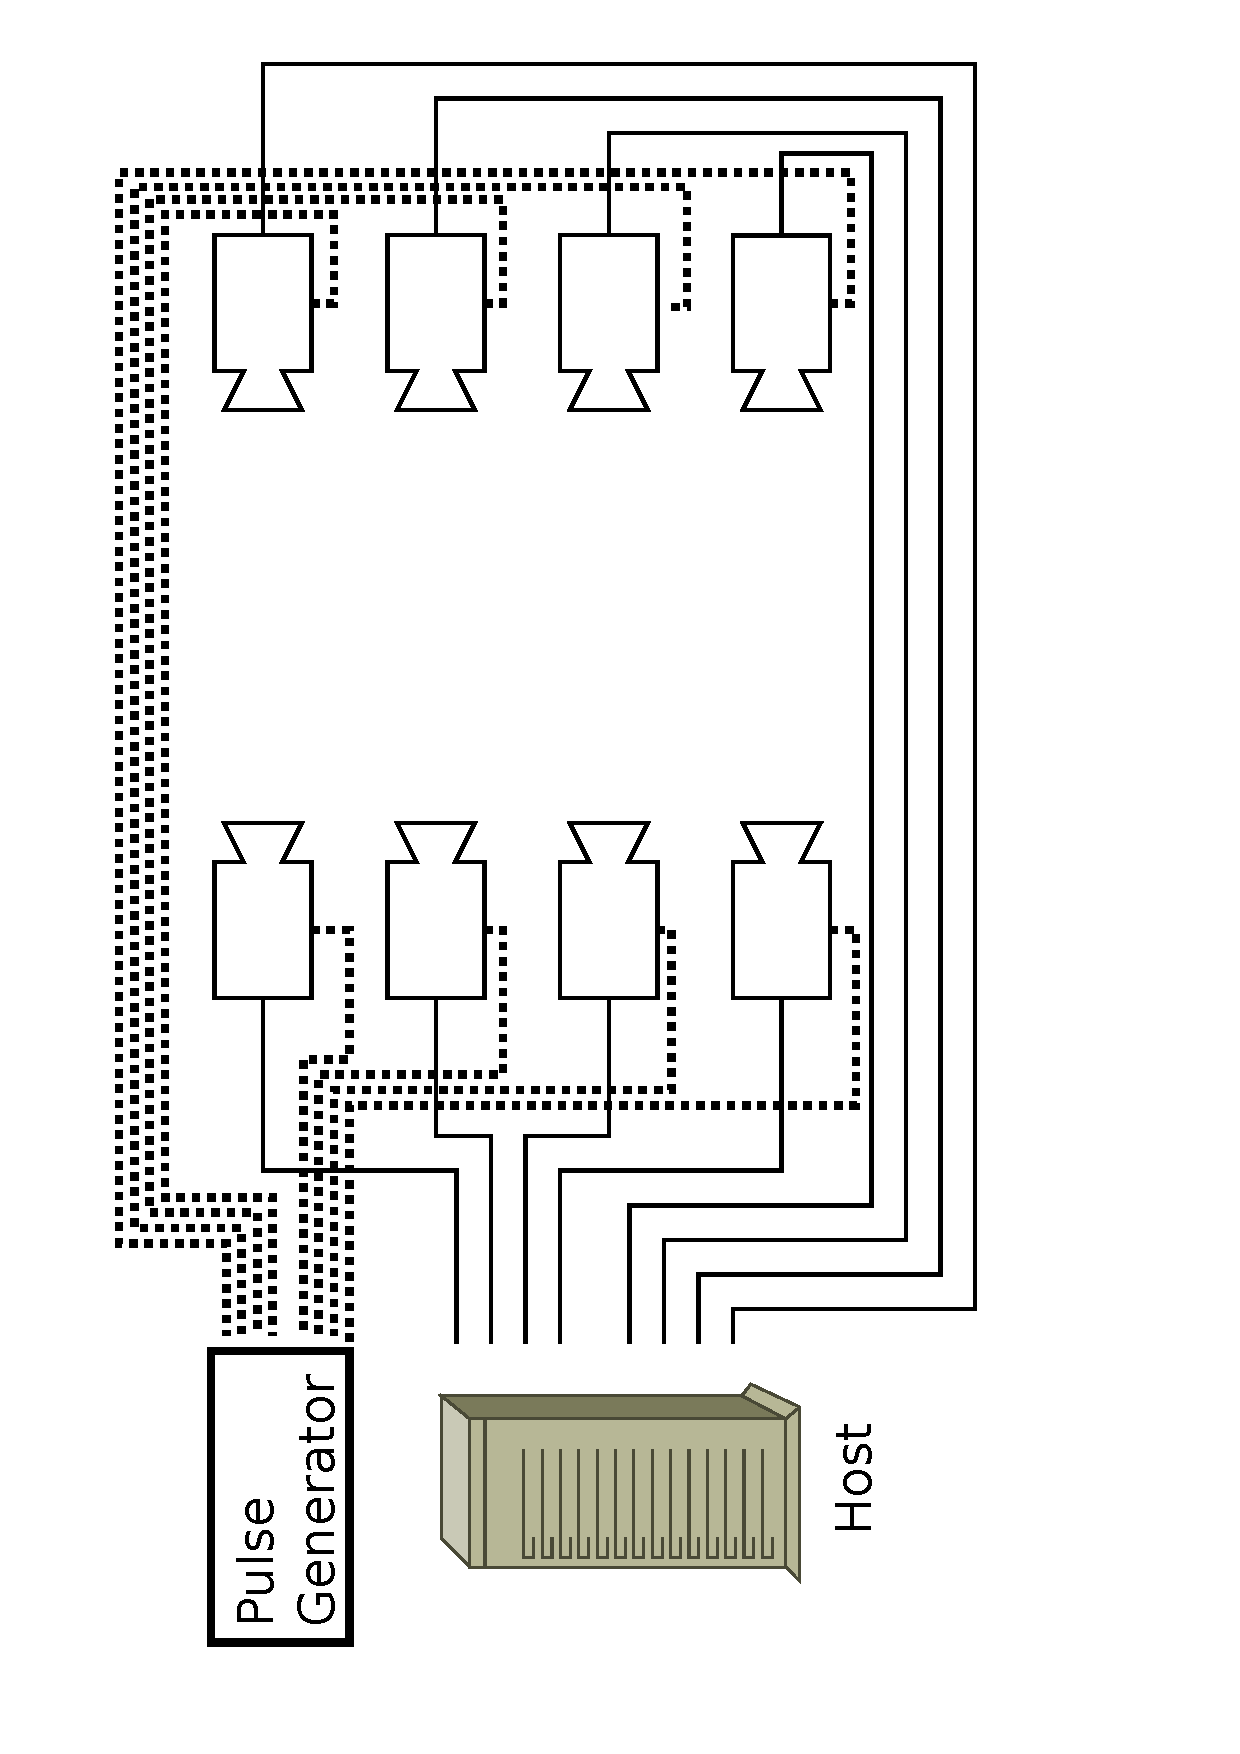
\includegraphics[angle=-90,width=\linewidth]{figures/ip_cameras.pdf}
        \caption{Eight FLIR/PointGrey IP cameras are directly
          connected via Gigabit Ethernet (GigE) directly to two 4-port
          network cards at the host. An external pulse generator
          (PixHawk) is used to trigger the cameras.}
    \label{fig:gige_setup}
\end{figure}
In this section we briefly go over the hardware setup, shown in
Fig. \ref{fig:gige_setup},  with which the experimental data was collected.

Eight Gigabit Ethernet color cameras (FLIR BFLY-PGE-23S6C-C) are located
up to about 7m apart and are facing each other. The cameras utilize a 1" Sony
Pregius IMX249 global shutter sensor which offers an image resolution of
1920x1200 at up to 41 Hz. Shielded CAT6E twisted pair copper cables
transport the data over a 
distance of about 15m to a central host. The camera shutters are
triggered synchronously at 40Hz (1ms strobe duration) by an external pulse generator, in
this case a PixHawk running the PX4 flight stack, which has a feature
to generate an external TTL pulse at 3.3V.

\begin{figure}[h]
	\centering
	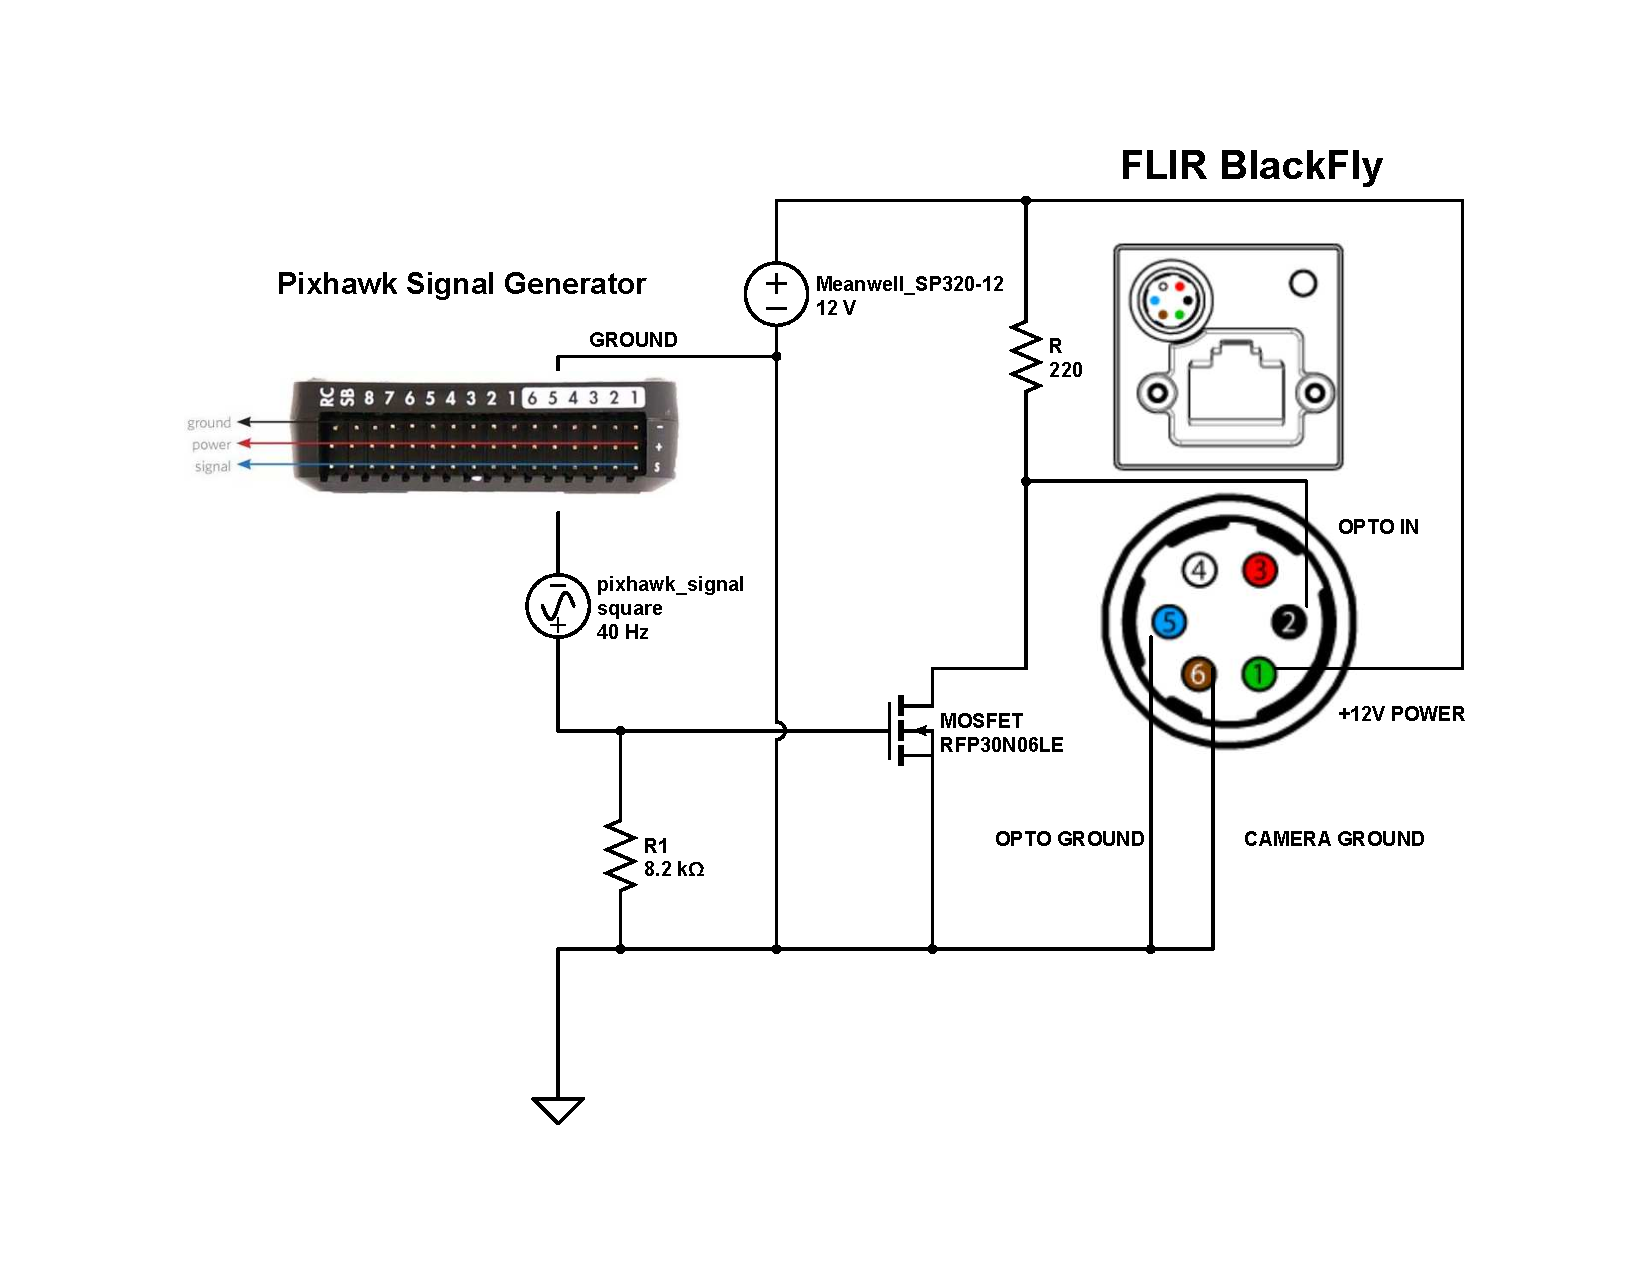
\includegraphics[width=\linewidth]{figures/aviary_sync_circuit.pdf}
        \caption{Circuit for driving the GPIO sync pin of eight FLIR/PointGrey Blackfly
          cameras from a PixHawk 3.3V TTL pulse. The signal is too
          weak to drive the eight opto-coupled input ports of the
          cameras, and is therefore amplified by a TTL MOSFET.}
    \label{fig:sync_circuit}
\end{figure}

Unfortunately, the signal from the PixHawk is not strong enough to
drive all eight camera input pins. The required amplifier circuit is
shown in Figure \ref{fig:sync_circuit}. In this configuration, the
signal to the cameras has a peak of 6V, which is well above the 3V
required to drive the opto coupler. If more 
cameras are connected and the signal gets too weak, a 
smaller resistor R should be used.

When running at 40Hz, transmitting a camera's raw Bayer
images will already consume 737Mbits, not including network packet
overhead. This is just within the capacity of a 1Gbit link, and will
put signficant load on camera, network card, and host driver.
